\documentclass[10pt,a4paper,twocolumn,twoside]{article}
\usepackage[utf8]{inputenc}
\usepackage[english]{babel}
\usepackage{graphicx}
\usepackage{fancyhdr}
\usepackage{times}
\usepackage{titlesec}
\usepackage{multirow}
\usepackage{lettrine}
\usepackage[top=2cm, bottom=1.5cm, left=2cm, right=2cm]{geometry}
\usepackage[figurename=Fig.,tablename=TAULA]{caption}
\usepackage{listings, ../common/listings-rust}

\graphicspath{ {img/} }

\lstnewenvironment{code}[1][]%
{
   \noindent
   \minipage{\linewidth} 
   \vspace{0.5\baselineskip}
   \lstset{language=Rust, style=colouredRust,#1}}
{\endminipage}

\author{\LARGE\sffamily Josep Maria Domingo Catafal}
\title{\Huge{\sffamily  Design and implementation of a programming language with LLVM }}
\date{}

\newcommand\blfootnote[1]{%
  \begingroup
  \renewcommand\thefootnote{}\footnote{#1}%
  \addtocounter{footnote}{-1}%
  \endgroup
}

\titleformat{\section}
{\large\sffamily\scshape\bfseries}
{\textbf{\thesection}}{1em}{}

\begin{document}

\fancyhead[LO]{\scriptsize AUTOR: TÍTOL DEL TREBALL}
\fancyhead[RO]{\thepage}
\fancyhead[LE]{\thepage}
\fancyhead[RE]{\scriptsize EE/UAB TFG INFORMÀTICA: Design and implementation of a programming language with LLVM}

\fancyfoot[CO,CE]{}

\fancypagestyle{primerapagina}
{
   \fancyhf{}
   \fancyhead[L]{\scriptsize BACHELOR'S THESIS IN COMPUTER SCIENCE, ESCOLA D'ENGINYERIA (EE), UNIVERSITAT AUTÒNOMA DE BARCELONA (UAB)}
   \fancyfoot[C]{\scriptsize Febrer de 2023, Escola d'Enginyeria (UAB)}
}

\renewcommand{\headrulewidth}{0pt}
\renewcommand{\footrulewidth}{0pt}
\pagestyle{fancy}

\twocolumn[\begin{@twocolumnfalse}

\maketitle

\thispagestyle{primerapagina}

\begin{center}
\parbox{0.915\textwidth}
{\sffamily

    \textbf{Abstract--} This thesis presents the design and development of a new
    programming language called \textit{Craft}, using Rust and LLVM. The goal of
    the project is to gain a deeper understanding of how compilers work by
    creating one from scratch using these tools. The language is designed to be
    simple and easy to understand, but at the same time, it aims to be fast and
    efficient, so some sacrifices have to be made. The thesis covers the design
    and implementation of the language, including the lexer, parser, and code
    generation. The project also includes a discussion of the challenges
    encountered during development and suggestions for future work. Overall, the
    project serves as a valuable learning experience for understanding the inner
    workings of compilers and the capabilities of Rust and LLVM.

    \bigskip

    \textbf{Keywords-- } Programming Language, LLVM, SSA, Strongly Typed, Compiled

    \bigskip

    \textbf{Resum--} Resum del projecte, màxim 10 línies.

    \bigskip

    \textbf{Paraules clau-- } Llenguatge de programació, LLVM, SSA, Fortament tipat, Compilat
}
\end{center}

\bigskip
\end{@twocolumnfalse}]

\blfootnote{$\bullet$ E-mail de contacte: jdomingocatafal@gmail.com}
\blfootnote{$\bullet$ Menció realitzada: Computació}
\blfootnote{$\bullet$ Treball tutoritzat per: Javier Sanchez Pujadas (Ciències de la Computació)}
\blfootnote{$\bullet$ Curs 2022/23}

\section{Introduction}
\lettrine[lines=3]{H}{istorically}, there has always been a dilemma between the
speed of execution, and speed of development. Some languages are easy to
program: they allow the programmer to not worry about low-level concepts such as
memory management, and create abstractions that streamline the development. The
problem is that these abstractions limit language efficiency, and create slower
programs. Another reason that allows speeding up development is dynamic typing,
as it frees the user from the mental overhead that comes with deciding the type
that should be used. But this also has its own disadvantages, since it is very
likely that you will encounter errors in timing of execution These languages
tend to be interpreted in order to save money it waits for the programmer, but
it has an impact on the execution performance of the program if we compare it to
compiled languages. Python, for example, would be one of the largest
representatives of this group of languages. On the other side of the currency
and we have languages like C, which have almost no abstraction and the
programmer must be aware of what he is doing in every line of code he writes.
they are languages that provide very good performance, but slow down the
development, as the programmer must take into account many concepts of low level
An additional problem is that when managing shape memory manual, it opens the
door to a lot of runtime errors in the form of memory leaks. Currently, there
are languages like Rust that solve this these memory management issues without
losing performance, but the development is still slow and the compilation time
long. these languages tend to be strongly typed, which reduces errors in
runtime, but slows down development.

\section{Goals}

\section{State of the art}
\subsection{Programming Languages}
\subsection{Compilers}

\section{Methodology}

\section{Tech Stack}

Writing a compiler does not require many tools, but some of them can help a lot
in paving the road. For this compiler we are going to use two tools: 
The Rust Programming Language and LLVM.

We are also going to use two tools for managing the source code: Git with GitHub
for hosting.

\subsection{Rust}
Rust is a systems programming language that was first released in 2010. It was
developed by the Mozilla Foundation with the goal of creating a safe and
concurrent language that would be suitable for low-level systems programming
tasks, such as operating systems, and performance critical programs, like a
browser engine. One of the major features of the language is it's guaranteed
memory-safety (and thread-safety) without requiring the use of a garbage
collector or reference counting (and thus not compromising on performance).
This combined with its powerful type system, help catch a lot of bugs at 
compile-time.

For this reasong we are going to use this language. It's also really comfortable
to use and comes with a lot of great tooling like cargo, which is the command 
line tool used for compiling, managing dependencies, etc. and clippy, a linter
that comes built in and gives great hints on how to improve the code.

\subsection{LLVM}
LLVM is a tool chain for building compilers, i.e. a set of tools different ones
that help us in implementing compilers. It was created in 2003 by Chris Lattner
(also creator of the Swift programming language) and has the support of
companies like Apple (LLVM is a part integral part of XCode and Swift for iOS
application development), Google, IBM or Intel. Currently, there are several
mainstream programming languages that use it, such as C/C++ (via the Clang
compiler, a alternative to GCC), Rust, Swift, Crystal...

As we said LLVM has a lot of tools, but among all them, the LLVM Core libraries
are the most important and particularly relevant for us. 

We will be referring to 
them as LLVM from now on for simplicity. 

LLVM will allow us to generate assembly for a lot of different architectures
without any extra effort. It can even generate Web Assembly, which allows us to
run the language in modern web browsers. The Craft compiler will generate LLVM
IR (Intermidiete Representation), and then it will be piped to LLVM, which will
take the IR, apply transformations to it, in order to optimize it, and then
the assembly for the target architecture will be generated.

Generating LLVM IR instead of assembly, also frees us from some headaches. For
example, since LLVM is architecture independent, when we generate the code, we
don't we need to worry about the number of registers, as we have an unlimited
number of virtual registers, which LLVM will later map to the registers of the
corresponding architecture.

As we discussed, LLVM also applies optimizations to the generated code, like
dead code elimination, constant folding, loop unrolling, etc. However, in order
for LLVM to perform these optimizations, we will have to generate the code in
SSA (Static single-assignment). This means that we can only assign a value to a
variable once. If we need to reassign a value, a new variable has to be created
that replaces the other one. The reason SSA is used is because it makes 
applying optimizations a lot easier.

\section{Git and GitHub}
For version control Git was chosen since it's the industry standard and one of
the most powerful tools out there. The repo is hosted on GitHub which is great
for open source projects and allows us to use GitHub Actions. The repository is 
configured such as that on every Pull Request or commit to the master branch,
a GitHub action runs that compiles the code, runs Clippy, runs the tests and 
checks the formatting of the code. This way we prevent broken code to enter the
stable branch.

\section{Development}
\section{Architecture}
Most compilers are divided into two parts: the front-end and the back-end. The
front-end is the part of the compilers that takes the source code and transforms
it into an intermediate representation than will later be transformed into the
actual machine code by the back-end. In our case, since we are using LLVM, we
don't need to worry too much about the back-end, since LLVM will be in charge of
generating the machine code. Out job will be to go from the source code to the
LLVM intermediate representation (we will call it \textbf{\textit{IR}} from now
on). The front-end of the compiler is typically composed of three main steps.

\begin{figure}[ht]
\centering
\captionsetup{justification=centering,margin=1cm}
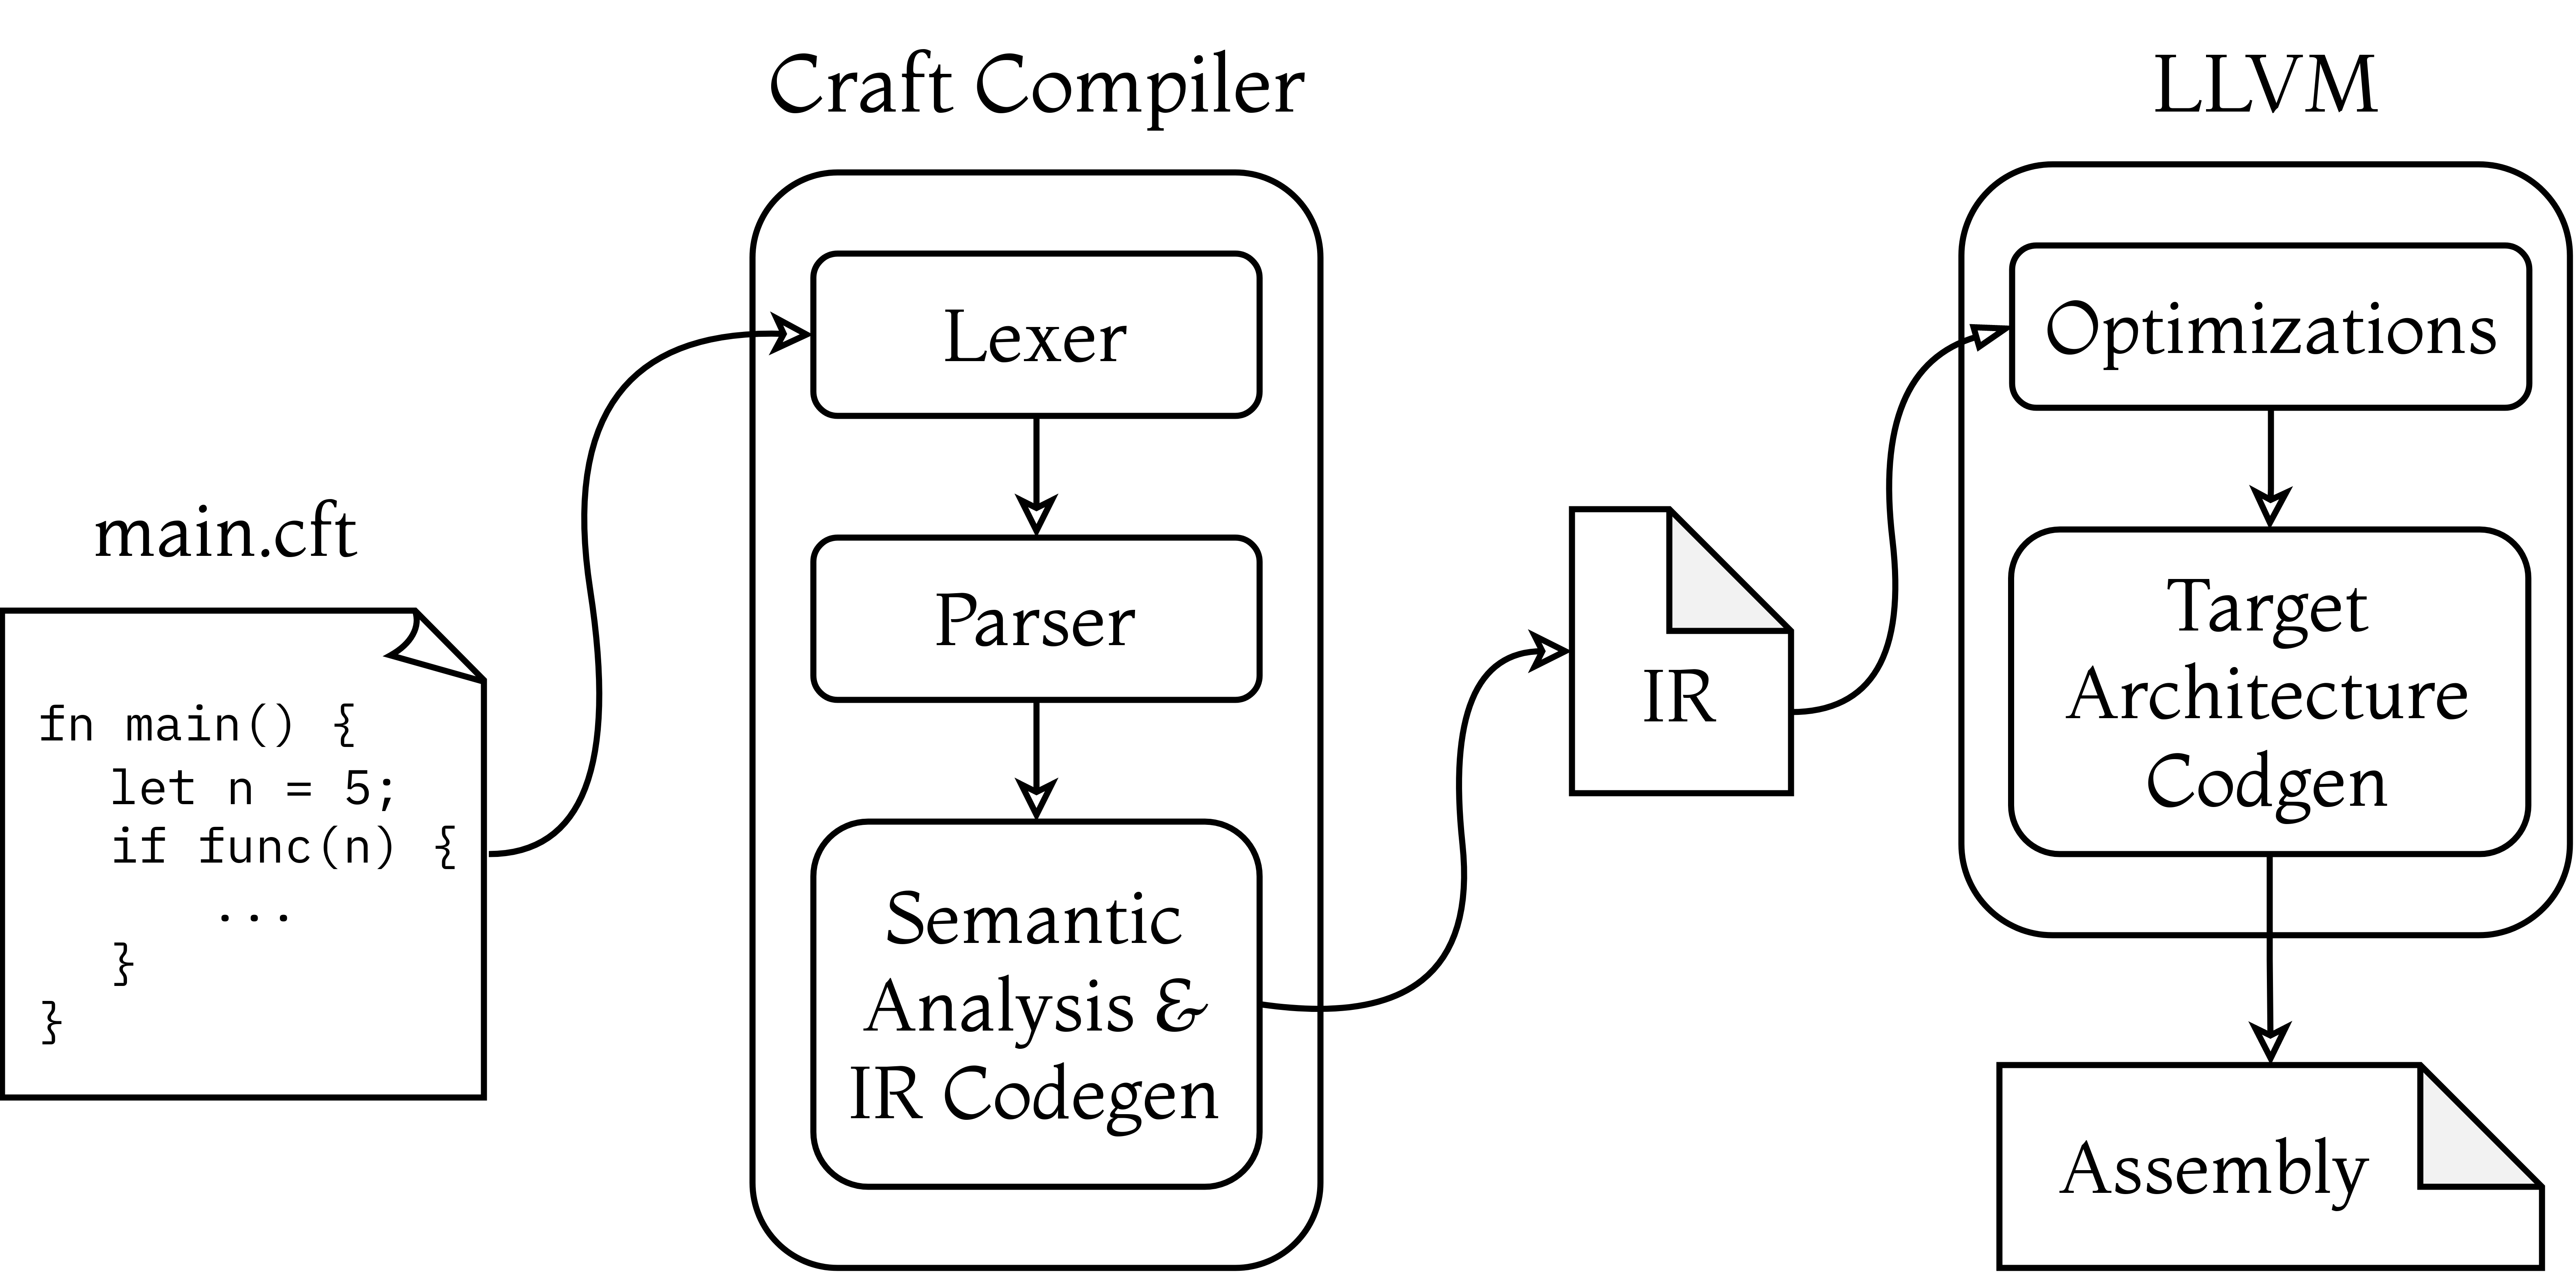
\includegraphics[width=\linewidth]{arch}
\caption{Diagram showing the compilation workflow of a Craft program}
\end{figure}

\subsection{Lexing} 
This step consists of breaking the source code into a sequence of tokens. A
token is a basic building block of the languages, such as a keyword or an
identifier.

A lexer can be implemented rather easily, by using a state machine. An approach
to do it programmatically could be the following:

\begin{enumerate}
    \item Start by reading the source code character by character until we reach
        the end.
    \item If the character by itself forms a valid sequence (e.g. a parenthesis)
        we create a token from it. If it doesn't, we continue reading characters
        until we find a valid sequence. 
\end{enumerate}

Note that sometimes we may find a valid sequence, but that's not enough to
create a token, since it may be the start of another longer and valid sequence.
We may need to check the following character/s to check weather it continues. An
example of such case would be the '\texttt{>}' operator, since, by itself is a
valid sequence, but it may be the start of the '\texttt{>=}' operator. So we
need to check if the next character is an '\texttt{=}' or something else.

The lexer requires a bit of work to set up, but after that, expanding it is 
trivial, since we only need to add a new word to the list of reserved words, in 
the case we want to add a reserved word, or add a new rule that detects a new 
symbol for example.


\subsection{Parsing}
The lexer allowed us to identify the simbols of the program, but it does not 
allow us to determine if their order is correct, or if they follow the rules of
the language (i.e. it's grammatically correct). That is the job of the parser.

The parser takes the sequence of tokens obtained from the lexer and
transforms it into an Abstract Syntax Tree (AST). This tree represents the
structure of the program and determines its syntactic structure. It will tell us
the order in which we need to execute the instruction.

To generate the AST compilers use a context free grammar. A grammar is a set of
rules that tells us how to form valid strings of tokens in a specific language.
They are formed of a set of symbols, which can be divided into terminal and
non-terminal symbols, and a set of production rules that specify how the
non-terminal symbols can be replaced by sequences of terminal and non-terminal
symbols. A context free grammar is a type of grammar that, the rules of the grammar do
not depend on the context in which the symbols appear.

The goal of the parser is to make the program obey the rules of the grammar.

Here's an example of a simple grammar for parsing function prototypes:

\begin{small}
\begin{verbatim}
<proto>   ::= fn <id> "(" <params> ")"
<id>      ::= letter {letter | digit | "_"}
<params>  ::= "("{ <param> {, <param> } }")"
<param>   ::= <id>: <type>
\end{verbatim}
\end{small}

If we were to translate the proto rule to code, it would look something like 
this:

\begin{scriptsize}
\begin{code}
fn parse_prototype() -> (Prototype, Err) {
    // we expect to find the fn keyword,
    // else it's an error
    match current_token().kind {
        // The advance function moves to the next token
        TokenKind::Fn => advance(),
        _ => return Err("Expected fn keyword"),
    };

    // we expect to find the function name,
    // else it's an error
    let name = match current_token().kind {
        TokenKind::Identifier => current_token().lexeme,
        _ => return Err("Expected an identifier"),
    };

    advance();

    // we call the params rule
    let params = parse_params();

    // we are done, we return a struct 
    // with the info of the prototype
    return Prototype { 
        name,
        params,
    };
}
\end{code}
\end{scriptsize}

\subsection{Semantic Analysis and [IR] Code Generation}
Once we have an AST, we can traverse it to generate the LLVM IR. Since this is a
simple compiler, we are going to do the semantic analysis in this step. With 
more complex compilers, we may want to create a specific step of semantic 
analysis, but in out case it is not necessary.

LLVM has the concept of modules. A module contains all the information
associated with one code file. If we have multiple files, we simply have to
create different modules and link them. Modules contain functions and functions
are made up of instructions, similar to the instructions we find in assembly.

Let's see an example of a small piece of code and what it would look like in the
intermediate representation of LLVM. We have the following function that
receives two integers and returns the maximum:

\begin{code}
fn max(int a, int b) int {
    if a > b { a } else { b }
}
\end{code}

If we translate it to LLVM IR we have the following code:

\begin{scriptsize}
\begin{code}
define i32 @max(i32 %a, i32 %b) {
entry:
  %0 = icmp sgt i32 %a, %b
  br i1 %0, label %btrue, label %bfalse

btrue:
  br label %end

bfalse:
  br label %end

end:
  %retval = phi i32 [%a, %btrue], [%b, %bfalse]
  ret i32 %retval
}
\end{code}
\end{scriptsize}

The first line of the previous code defines a function, which receives two
32 bits integers. A label entry is defined below. These tags are like assembly
tags, and we can jump to them.

The first thing it does, on the 'entry' tag, is comparing both integers (i.e.
the if condition). The \texttt{'sgt'} keyword, means 'signed greater than',
which, as the names says, does a greater than signed comparison. The result of
the comparison is a one bit integer which acts like a boolean. If it's true, it
will jump to the label \texttt{btrue}, otherwise to the label \texttt{bfalse}.

In this case the two branches do the same thing: a jump to the label
\texttt{end}. There we come across a concept called phi nodes. The phi nodes
are kind of an inverted if. Depending on where we did the jump we will assign
one value or another to the variable \texttt{retval}. If we come from
\texttt{btrue}, \texttt{retval} is assigned \texttt{\%a}, and if we come from 
\texttt{bfalse} it is assigned to \texttt{\%b}.

Now, why do the two branches jump to the \texttt{end} tag and then do a
conditional again in the \texttt{end} block? Couldn't we assign the value of
\texttt{retval} directly inside the branch \texttt{btrue} or \texttt{bfalse} and
spare us that third conditional? Well the answer is no, because then we would be
generating code that is not in SSA form. And as we mentioned earlier, LLVM
requires the generated code to be in SSA form. And that's why phi nodes exist,
to be able to solve this types of problems.

\subsubsection{LLVM API}


\section{Results}
\section{Conclusions}

\begin{thebibliography}{11}
\bibitem{latex}
http://en.wikibooks.org/wiki/LaTeX

\bibitem{2}
Referència 2

\bibitem{3}
Etc.

\end{thebibliography}

\appendix

\section*{Apèndix}

\setcounter{section}{1}

\subsection{Secció d'Apèndix}
.... ... ..... ... ..... ... ... ..... .... .

\subsection{Secció d'Apèndix}
.... ... ..... ... ..... ... ... ..... .... .

\end{document}
